\begin{ledgroupsized}[r]{120mm}%
\footnotesize%
\pstart%
\noindent\textbf{\"{U}berlieferung:}%
\pend%
\end{ledgroupsized}%
\begin{ledgroupsized}[r]{114mm}%
\footnotesize%
\pstart%
\parindent -6mm%
\makebox[6mm][l]{\textit{L}}%
Auszüge mit Bemerkungen aus einem nicht weiter identifizierten Manuskript von Acar:
LH~III~4,~8a Bl.~1.
1 Bl. 2\textsuperscript{o}. 1 S. auf Bl.~1~r\textsuperscript{o}.
Bl.~1~v\textsuperscript{o} leer%, bis auf ein \textit{a}, vermutlich nicht von Leibniz
. Ein Wasserzeichen.%
\newline%
Cc 2, Nr. 1563%
\pend%
\end{ledgroupsized}%
%
\vspace*{5mm}%
\begin{ledgroup}%
\footnotesize%
\pstart%
\noindent%
\footnotesize{%
\textbf{Datierungsgr\"{u}nde:}
Das Wasserzeichen im Textträger des vorliegenden Stücks N.~74 % LH003,04,08a_001
ist für einen Zeit\-raum belegt, welcher das Jahr 1675 und die erste Hälfte des Jahres 1676 umfasst.
Da weitere Anhalts\-punk\-te für eine genauere chronologische Einordnung fehlen,
wird dieser gesamte Zeitraum als Datierung von N.~74 %
vorgeschlagen.}%
\pend%
\end{ledgroup}%
%
%
\vspace{6mm}%
\count\Bfootins=1200
\count\Cfootins=1200
\count\Afootins=1200
\pstart%
\normalsize%
\noindent%
% [1~r\textsuperscript{o}]
[1~r\textsuperscript{o}] 
\edtext{%
Secrets Medicinaux considerables, et pour la plus part \'{e}prouuez
\edtext{tirez d'un liure}{\lemma{tirez}\Bfootnote{\textit{(1)} d'un MS \textit{(2)} d'un liure \textit{L}}}
in 8\textsuperscript{o} \'{e}crit de la main de feu Mons. Acar,\protect\index{Namensregister}{\textso{Acar} bzw. Acart, ???? ??-??}
homme tres exact, et qui faisoit des experiences.%
}{\lemma{Secrets [...] experiences}\Cfootnote{%
Ein \textit{Mons. Acar} (bzw. \textit{Acart}) wird in der Literatur der Zeit als Naturforscher im Umfeld der sog. \glqq Académie Bourdelot\grqq~dargestellt;
siehe etwa \cite{01149}\textsc{P.\,M. Bourdelot}, \textit{Conversations académiques}, Paris 1672, S.~59 und S.~71.
Leibniz hat offenbar Gelegenheit gehabt, ein kleinformatiges Manuskript von ihm zu exzerpieren.}}%
%
\pend%
\pstart%
\textso{Recette infallible pour les hemorroides.}\protect\index{Sachverzeichnis}{h\'{e}morro\~{i}des}
Faut porter sur soy deux ou trois petites noisettes, ou fruits, qui se trouuent dans la teste du chardon\protect\index{Sachverzeichnis}{chardon} sauuage ou b\^{a}tard, qui croist dans les champs. Il y a des petits vers dans les dites petites noisettes, les quels tant qu'ils vivent garantissent du mal: ils vivent pr\'{e}s d'un an, c'est pourquoy les faut changer quand ils meurent
\edtext{\lbrack+}{\lemma{\lbrack+}\Cfootnote{Eckige Klammer von Leibniz.}}%
~cela ne paroist vraysemblable. Mais il faut que Mons. Acar\protect\index{Namensregister}{\textso{Acar} bzw. Acart, ???? ??-??}
l'ait ou essay\'{e}, ou appris d'une personne dont la relation ne luy estoit pas suspecte. Sans cela il ne l'auroit pas mis, avec le titre d'infallible, parmy une trentaine de receptes choisies~%
\edtext{+\rbrack.}{\lemma{+\rbrack}\Cfootnote{Eckige Klammer von Leibniz.}}
\pend%
\pstart%
\textso{Pour le mal caduc.}\protect\index{Sachverzeichnis}{mal caduc}
Mons. Garillon\protect\index{Namensregister}{\textso{Garillon}, ????, ??-??}
le fils Chevalier de Malthe, qui demeure chez lonpere (+~ou tonpere~+) procureur, vers S. C\^{o}me dans la rue de la harpe, a une pierre, la quelle si tost qu'elle touche celuy qui est tomb\'{e} du mal, revient aussi tost.
\pend%
\pstart%
\textso{Pour la dysenterie.\protect\index{Sachverzeichnis}{dysenterie}}
Faut prendre trois pintes de gros vin\protect\index{Sachverzeichnis}{vin} rouge, le faire bouillir \`{a} petit feu, dans un pot de terre neuf, et y mettre dedans plein les deux mains de chardon\protect\index{Sachverzeichnis}{chardon} volant coup\'{e} par petits morceaux. Le nettoyer sans le laver, et le laisser au feu tant que le dit vin\protect\index{Sachverzeichnis}{vin} ne devienne qu'\`{a} un demy septier, puis faire mettre le malade aupres du feu, et le frotter du dit vin\protect\index{Sachverzeichnis}{vin}, le plus chaud qu'il pourra souffrir, d\'{e}puis le col tout du long de l'\'{e}pine du dos, jusqu'au fondement, et aprez le faire coucher dans le lict sur le dos, ayant mis des linges bien chauds, le long de l'\'{e}pine, puis mettre le dit vin\protect\index{Sachverzeichnis}{vin} d\'{e}puis le nombril jusqu'au fondement, et y mettre des linges chauds.
\pend%
\pstart%
\textso{Pour la blessure d'une saign\'{e}e.}\protect\index{Sachverzeichnis}{saign\'{e}e}
Faut mettre sur la playe une mie de pain mollet tout chaud tremp\'{e} dans du vin\protect\index{Sachverzeichnis}{vin} blanc.
\pend%
\pstart%
\textso{Pour le cours de ventre.}
Faut mettre dans deux cuiller\'{e}es d'huyle d'olive, et deux cuiller\'{e}es d'eau rose;\protect\index{Sachverzeichnis}{eau de rose}
une cuiller\'{e}e de sucre, et battre tout ensemble, et le prendre \`{a} jeun, et reiterer deux ou trois fois; jusqu'\`{a} ce qu'on en soit soulag\'{e}.
\edtext{De}{\lemma{De}\Bfootnote{\textit{erg. L}}}
Mademoiselle de la Haye\protect\index{Namensregister}{\textso{Mademoiselle de La Haye 1580-1651}
illegitime Tochter Louis III de Guise, Kardinal in Reims ??}.
\pend%
\pstart%
\textso{Pour le mal de cost\'{e}}\protect\index{Sachverzeichnis}{mal de c\^{o}t\'{e}}\textso{ ou pleuresie.}\protect\index{Sachverzeichnis}{pleur\'{e}sie}
Faut fricasser de l'avoine\protect\index{Sachverzeichnis}{avoine} avec une cuiller\'{e}e de vinaigre, puis la mettre dans un sachet, et l'appliquer sur le cost\'{e}, le plus chaud que l'on puisse. De Mademoiselle de Luzancourt.\protect\index{Namensregister}{\textso{Mademoiselle de Luzancourt}, ???? ??-??}
\pend%
\pstart%
\textso{Pour la goutte.}\protect\index{Sachverzeichnis}{goutte}
Faut mettre pour 1 sol de couperose\protect\index{Sachverzeichnis}{couperose} verte dans une pinte d'urine; bouillir \`{a} la moiti\'{e}; en mouiller un linge du quel on s'enveloppera deux nuits. De Mademoiselle de Luzancourt.\protect\index{Namensregister}{\textso{Mademoiselle de Luzancourt}, ???? ??-??}
\pend%
\pstart%
\textso{Pour la douleur des yeux.}\protect\index{Sachverzeichnis}{douleur des yeux}
Faut piller des feuilles de tref (+~puto trefle\protect\index{Sachverzeichnis}{tr\`{e}fle}~+), marqu\'{e}e  \protect\rule[-3mm]{0mm}{14mm}\raisebox{-1mm}{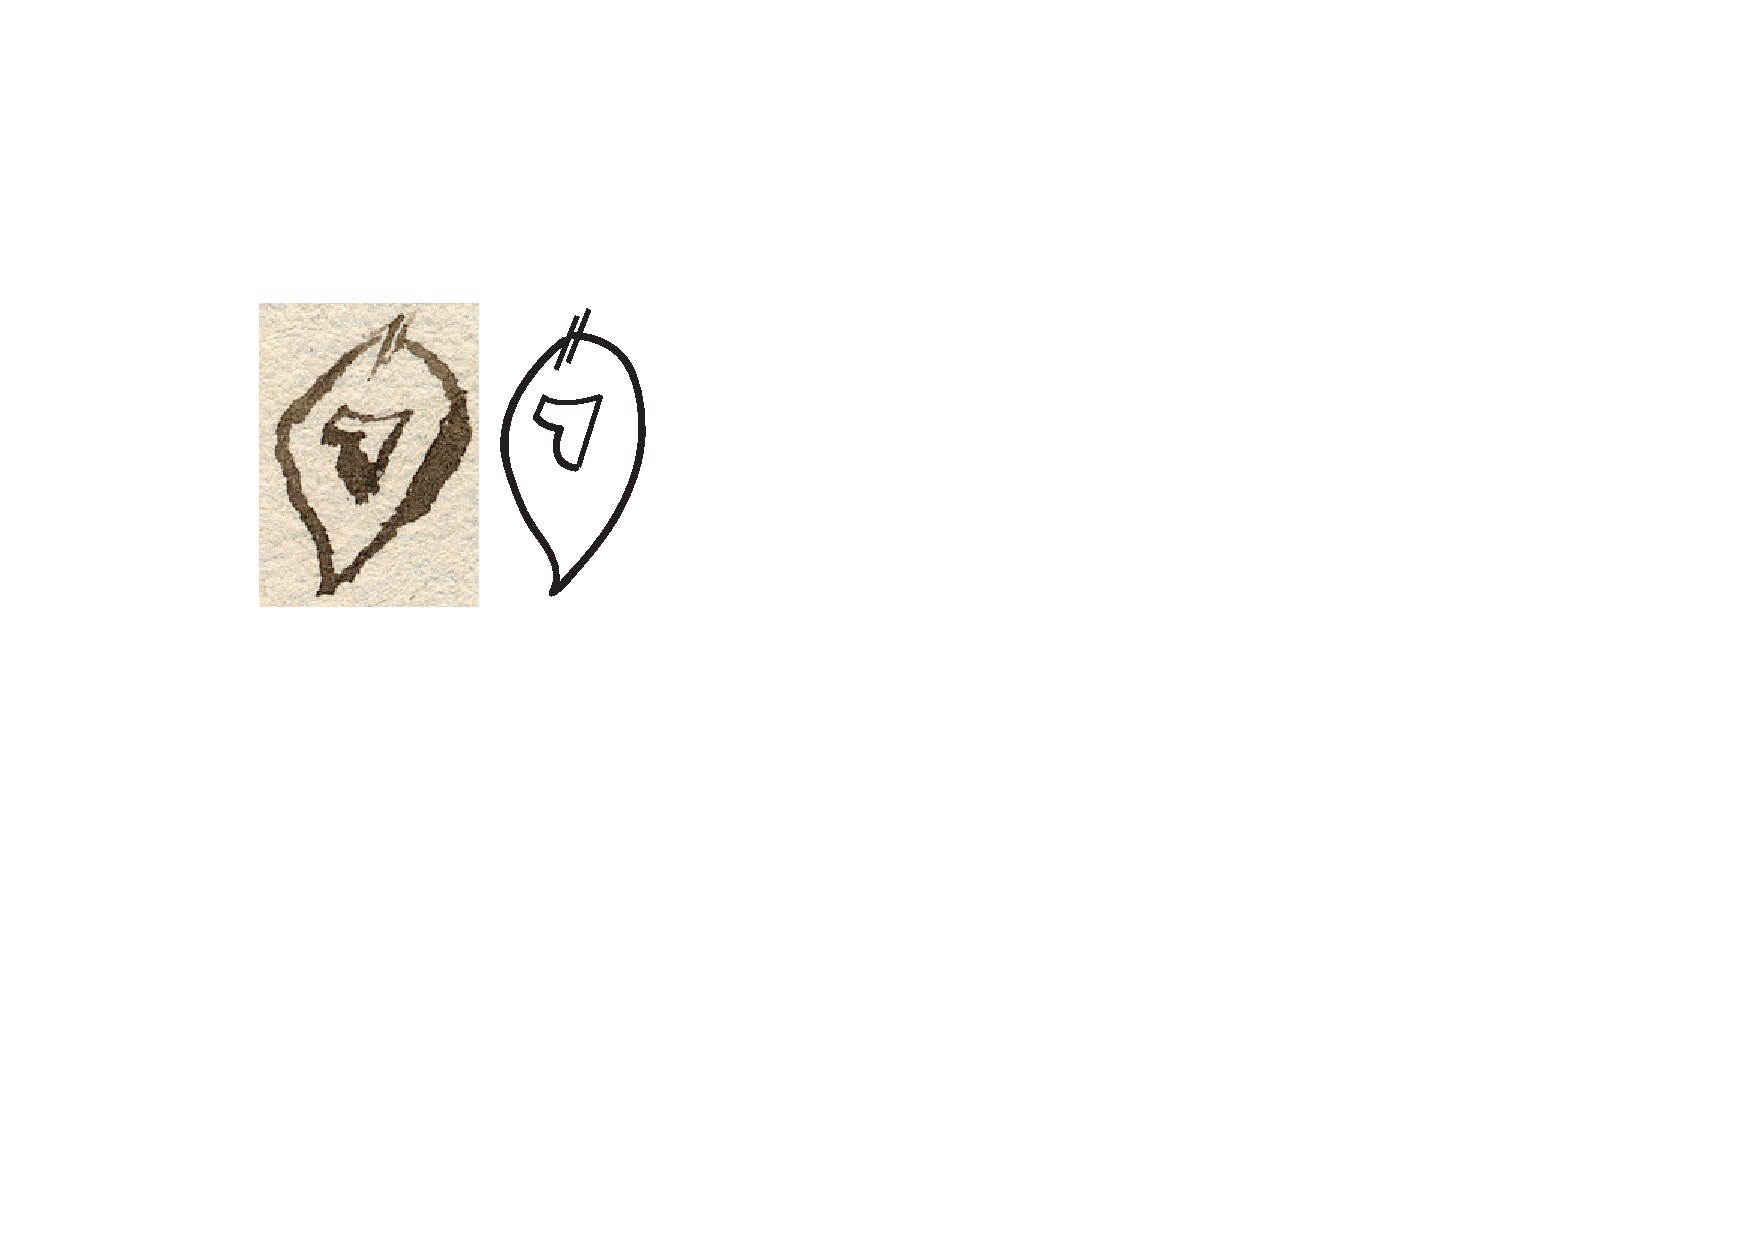
\includegraphics[width=0.1\textwidth]{images/lh0030408a_001r-draw1c.pdf}} qui vient dans les champs, et en mettre le jus dans les yeux pendant 7 ou 8 jours.
\pend%
\pstart%
\textso{Pour la bruslure.}\protect\index{Sachverzeichnis}{br\^{u}lure}
L'ail\protect\index{Sachverzeichnis}{ail} distill\'{e} y est excellent.
\pend%
\pstart%
\textso{Pour l'asthme}\protect\index{Sachverzeichnis}{asthme}%\edlabel{acar5}
\textso{ ou \'{e}touffement.}\protect\index{Sachverzeichnis}{\'{e}touffement}
Faut mettre une dragme de souffre\protect\index{Sachverzeichnis}{soufre} crud pulveris\'{e}, et l'avaller dans un verre de vin\protect\index{Sachverzeichnis}{vin}. Le blanc est le meilleur. La tinture de souffre\protect\index{Sachverzeichnis}{tinture de soufre} est excellente.
\pend%
\pstart%
%\edtext{}{{\xxref{acar5}{acar6}}\lemma{}\Bfootnote{\textit{Am rechten Rand der Abs\"{a}tze zu Asthma drei Klammern. Die erste fasst die zwei S\"{a}tze} Demy douzaine [...] purgent doucement. \textit{zusammen, die zweite die Abs\"{a}tze} Autre remede [...] quam Vafor +). \textit{und die dritte} \textso{Pour l'Asthme} [...] quam Vafor +).}}
\textso{Recepte admirable pour l'asthme.}
Prenez de l'orge\protect\index{Sachverzeichnis}{orge} mond\'{e}e et la faites bouillir, comme si l'on la vouloit manger, cela fait, il la faut bien laver et piller dans un mortier, puis il faut la passer par un linge avec du laict du cheuure\protect\index{Sachverzeichnis}{lait de ch\`{e}vre}, si l'on en peut avoir; si non, faut se contenter du laict de vache\protect\index{Sachverzeichnis}{lait de vache}, le quel fait vous laisserez bouillir avec l'orge\protect\index{Sachverzeichnis}{orge} pass\'{e}e, jusqu'\`{a} ce qu'il devienne \'{e}pais, comme une bouillie, apres quoy
\edtext{vous la succrerez}{\lemma{vous la}\Bfootnote{\textit{(1)} succrez \textit{(2)} succrerez \textit{L}}}
bien, avec du sucre candy\protect\index{Sachverzeichnis}{sucre candi}; et vous la mangerez le matin et le soir, mais il ne faut pas boir apr\'{e}s. Ce secret est admirable aussi pour toutes sortes d'apostumes\protect\index{Sachverzeichnis}{apostume}, et on s'en est tousjours servi avec grand succ\'{e}s.
\pend%
\newpage
\pstart%
\textso{Autre:} un verre d'urine\protect\index{Sachverzeichnis}{urine} de soy, ou de quelqu'un qui soit bien sain est souuerain pour plusiers incommoditez principalement pour \textso{l'asthme.}\protect\index{Sachverzeichnis}{asthme}
\pend%
\pstart%
Le souffre\protect\index{Sachverzeichnis}{soufre} est excellent pour le \textso{poulmon}\protect\index{Sachverzeichnis}{poumon}.
\pend%
\pstart%
Demy\edlabel{acar3} douzaine de brignolles\protect\index{Sachverzeichnis}{prune de Brignoles} mangez le matin \`{a} jeun, sont fort bonnes.
\pend%
\pstart%
Une vingtaine de roses de muscat\protect\index{Sachverzeichnis}{muscat}, mangez \`{a} jeun, purgent \edlabel{acar4}doucement.\edtext{}{{\xxref{acar3}{acar4}}\lemma{}\Afootnote{\textit{Neben dem Text% eine Klammer und
:} \lbrack Je\textsuperscript{[a]} croy que c'est aussi pour l'Asthme.\protect\index{Sachverzeichnis}{asthme}\rbrack\textsuperscript{[b]}\\
{\footnotesize \textsuperscript{[a]} \lbrack Je: Eckige Klammer von Leibniz.
\quad
\textsuperscript{[b]} l'Asthme.\rbrack: Eckige Klammer von Leibniz.%
}}}%
\pend%
\pstart%
Autre remede tres bon pour\textso{ l'asthme.}\protect\index{Sachverzeichnis}{asthme}
Prenez \edtext{palmonaria,\protect\index{Sachverzeichnis}{pulmonaria}}{\lemma{}\Afootnote{\textit{Über} palmonaria: puto: pulmonaria\protect\index{Sachverzeichnis}{pulmonaria}\vspace{-4mm}}}
hysope\protect\index{Sachverzeichnis}{hysope}, ana, une poign\'{e}e, d'anis\protect\index{Sachverzeichnis}{anis} et de fenouil\protect\index{Sachverzeichnis}{fenouil} ana, une cuiller\'{e}e; un bon baston de reglisse\protect\index{Sachverzeichnis}{r\'{e}glisse}, une cuiller\'{e}e de petits raisins\protect\index{Sachverzeichnis}{raisin}: et neuf figues\protect\index{Sachverzeichnis}{figue}, mettez le tout dans un pot de terre de deux pintes, et le remplissez avec de l'eau fra\^{i}che; et le laissez tout aupr\'{e}s du feu, jusqu'\`{a} ce qu'il soit bien \'{e}chauff\'{e}. Mais il ne faut pas le faire bouillir. Laissez le apres refroidir, et beuuez de cela un bon coup le matin, le soir, et toute la journ\'{e}e, quand vous voudrez, et autant que vous voudrez. Avec ce remede on a guery un homme, qui tomboit quelques fois comme mort, ne pouuant plus respirer.
\pend%
\pstart%
\textso{Pour se maintenir en sant\'{e}.}
Prenez deux dragmes de rubarbe\protect\index{Sachverzeichnis}{rhubarbe} de jardin, qui vient dans ce pays icy, raclez la dans du jus de pruneaux,\protect\index{Sachverzeichnis}{pruneau}
ou dans un bouillon, et le prenez \`{a} jeun le matin, elle est aussi fort bonne \`{a} manger \`{a} toute heure de la journ\'{e}e; on en fait aussi de la conserve.
\pend%
\pstart%
\textso{Excellante tisane}\protect\index{Sachverzeichnis}{tisane}%
\textso{ pour l'asthme.}\protect\index{Sachverzeichnis}{asthme}
Faut prendre un cacquemart de terre
\edtext{[+~topf~+]}{\lemma{[+~topf~+]}\Cfootnote{Eckige Klammern von Leibniz.}}
y mettre une pinte d'eau de fontaine et y faire bouillir une poign\'{e}e de son\protect\index{Sachverzeichnis}{son} bien sec, pour y mettre une cuiller\'{e}e de bon miel\protect\index{Sachverzeichnis}{miel} commun, qu'il faut bien ecumer en bouillant, et y mettre aussi un b\^{a}ton de reglisse\protect\index{Sachverzeichnis}{r\'{e}glisse} concass\'{e}; puis passer la dite tisane,\protect\index{Sachverzeichnis}{tisane} et en faire la
\edtext{[boisson].}{\lemma{boissons}\Bfootnote{\textit{L \"{a}ndert Hrsg.}}}
\pend%
\pstart%
Les gratteculs\protect\index{Sachverzeichnis}{gratte-cul} sont fort bons, que l'on peut manger \`{a} toute heure, les portant dans sa poche. Ces trois choses sont de Mademoiselle Bafor\protect\index{Namensregister}{\textso{Mademoiselle Bafort oder Vafor}, ???? ??-??}
(+~potius Bafor, quam Vafor~+)%\edlabel{acar6}.
\pend%
\pstart%
\textso{Recepte excellente contre la fieuure continue}\protect\index{Sachverzeichnis}{fi\`{e}vre continue}%
\textso{ et la peste.}\protect\index{Sachverzeichnis}{peste}
Prenez une poign\'{e}e de sel,\protect\index{Sachverzeichnis}{sel} un morceau de levain\protect\index{Sachverzeichnis}{levain} capable de couurir le front, deux cuiller\'{e}es du plus fort vinaigre\protect\index{Sachverzeichnis}{vinaigre}, et pour 3 sols de clous de girofle\protect\index{Sachverzeichnis}{girofle}. Et mettre le tout dans 
\pend
\newpage
\pstart\noindent un plat sur un r\'{e}chaud, qu'il faut un peu chauffer, et p\'{e}trir (kn\"{a}ten) ensemble; puis mettre la dite p\^{a}te entre deux linges, et l'appliquer sur le front, d'une
\edtext{temple, \`{a} l'autre,}{\lemma{}\Afootnote{\textit{Über} temple: tempora schlaff}}
qu'il faut renouueller
\edtext{quand il sera}{\lemma{}\Bfootnote{quand il\ \textbar\ sera \textit{gestr.}\ \textbar\ sera \textit{L}}}
sec, du matin \`{a} midy, ou du matin au soir. Les clous de girofle\protect\index{Sachverzeichnis}{girofle} peuuent reservir \`{a} diverses fois. Et continuer 2 ou 3 jours. Ce remede fait \textso{dormir} 10, 12, ou 14 heures.
\pend%
\pstart%
\textso{Pour garder le laict}\protect\index{Sachverzeichnis}{lait}%
\textso{ 5 ou 6 jours, fort bon.}
Faut, estant nouuellement tir\'{e} le faire bouillir un bouillon dans une terrine. Puis le mettre en lieu frais, et ne plus faire rechauffer. Il sera fort bon.
\pend%
\pstart%
Le crème de Normandie, qui se garde fort long temps, se tire au premier bouillon que l'on envoye dans des pots de grez, bien bouchez, \`{a} Paris.\protect\index{Ortsregister}{Paris}
\pend%
\pstart%
\textso{Pour la Gravelle.}\protect\index{Sachverzeichnis}{gravelle}
Faut faire bien seicher une \edtext{poign\'{e}e de tin}{\lemma{poign\'{e}e de}\Bfootnote{\textit{(1)} thin \textit{(2)} tin \textit{L}}}
(+~credo, thymus~+)
et une poign\'{e}e de sauge franche qui soit rouge, les mettre en poudre, tremper dans du vin\protect\index{Sachverzeichnis}{vin} blanc, puis le passer, et en prendre un ou 2 verres le matin.
\pend%
\pstart%
\textso{Remarque sur l'urine.}\protect\index{Sachverzeichnis}{urine}
Estant repos\'{e}e un jour, la rouge au fonds est bonne, la
\edtext{grise marque}{\lemma{grise}\Bfootnote{\textit{(1)} au \textit{(2)} marque \textit{L}}}
la gravelle\protect\index{Sachverzeichnis}{gravelle}, et la blanche marque la pierre\protect\index{Sachverzeichnis}{pierre (calcul r\'{e}nal>)}.
\pend%
\pstart%
\textso{Pour faire vuider la pierre.}\protect\index{Sachverzeichnis}{pierre (calcul r\'{e}nal)}
Faut prendre \`{a} jeun un verre ou demy verre, selon qu'on est robuste ou delicat, d'eau de racine de percil\protect\index{Sachverzeichnis}{persil} distill\'{e}e les carottes\protect\index{Sachverzeichnis}{carotte} fort bouillis, et pass\'{e}s. Est une tisane\protect\index{Sachverzeichnis}{tisane} fort bonne \`{a} boire \`{a} toute heure, pour la Pierre\protect\index{Sachverzeichnis}{pierre (calcul r\'{e}nal>)}.
\pend%
\pstart%
\textso{Pour la fieure tierce et la quarte.}\protect\index{Sachverzeichnis}{fi\`{e}vre tierce}\protect\index{Sachverzeichnis}{fi\`{e}vre quarte}
Prenez des amouraches\protect\index{Sachverzeichnis}{amourache} (qui est comme des petites marguerites\protect\index{Sachverzeichnis}{marguerite}) une poign\'{e}e, qu'il faut piller avec de la suif\protect\index{Sachverzeichnis}{suif} de chemin\'{e}e, une poign\'{e}e de sel\protect\index{Sachverzeichnis}{sel}, le blanc d'un oeuf\protect\index{Sachverzeichnis}{blanc d'oeuf} frais, puis mettre le tout ensemble, et le mettre entre deux linges, pour en faire un bracelet, qu'il faut appliquer au poignet. \textso{Autrement} prenez une poign\'{e}e de sel\protect\index{Sachverzeichnis}{sel}, de la suif\protect\index{Sachverzeichnis}{suif} de chemin\'{e}e, un oignon\protect\index{Sachverzeichnis}{oignon} blanc, un blanc d'oeuf\protect\index{Sachverzeichnis}{blanc d'oeuf}, et faites comme dessus. La rue\protect\index{Sachverzeichnis}{rue{??}} garantit des \textso{punaises}\protect\index{Sachverzeichnis}{punaise} mise par boucquets autour du lit.
\pend%
\pstart%
\textso{Purgation pour l'asme.}\protect\index{Sachverzeichnis}{acm\'{e}}
Faut mettre une chopine d'eau sur le feu, et la tirer
\edtext{[au]}{\lemma{eau}\Bfootnote{\textit{L \"{a}ndert Hrsg.}}}
premier bouillon, et y mettre aussi tost, le poids de deux \'{e}cus de sel\protect\index{Sachverzeichnis}{sel} de policreste\protect\index{Sachverzeichnis}{polycreste}, et le bien battre, en le versant d'un vaisseau en un autre, puis y mettre infuser du soir au matin un \'{e}cus de sen\'{e}\protect\index{Sachverzeichnis}{sen\'{e}}. Il faut prendre la dite chopine \`{a} jeun \`{a} matin, en deux fois \`{a} deux ou trois heures l'une de l'autre.
\pend%
\pstart%
Du frere Ange,\protect\index{Namensregister}{\textso{Fr{\`e}re Ange} capucin, duc de Joyeuse 1599-1608 ??} Capucin.
\pend%
\newpage
\pstart%
\textso{Pour rafraichir le sang.}
Dans quelque tisane\protect\index{Sachverzeichnis}{tisane} que ce soit d'orge\protect\index{Sachverzeichnis}{orge} de reglisse\protect\index{Sachverzeichnis}{r\'{e}glisse} ou autre, faut la tirant du feu toute bouillante y mettre deux poign\'{e}es de cerfeuil\protect\index{Sachverzeichnis}{cerfeuil}, une poign\'{e}e de pimpirnelle\protect\index{Sachverzeichnis}{pimprenelle}, et de chicor\'{e}e\protect\index{Sachverzeichnis}{chicor\'{e}e} sauuage la rend
\edtext{encore meilleure.}{\lemma{encore}\Bfootnote{\textit{(1)} plus \textit{(2)} meilleure. \textit{L}}}
Du frere Ange,\protect\index{Namensregister}{\textso{Fr{\`e}re Ange}, capucin, duc de Joyeuse 1599-1608 ??} Capucin.
\pend%
%\newpage
\pstart%
\textso{Pour la }\textso{fieure quarte.}\protect\index{Sachverzeichnis}{fi\`{e}vre quarte}
Prenez des raves\protect\index{Sachverzeichnis}{rave}, et les tranchez, et du sel.\protect\index{Sachverzeichnis}{sel}
Faites le bouillir dans un pot neuf, et les mettez dessous les pieds, et si une fois ne fait son effect, faut recontinuer.
\pend%
\pstart%
\textso{Pour la fieuure tierce.}\protect\index{Sachverzeichnis}{fi\`{e}vre tierce}
Prenez de l'encens\protect\index{Sachverzeichnis}{encens} male, du pain bis\protect\index{Sachverzeichnis}{pain bis}, de chacun une once et demy once de sel\protect\index{Sachverzeichnis}{sel}. Brisez le tout ensemble, et prenez du plus fort vinaigre\protect\index{Sachverzeichnis}{vinaigre}, pour enrouser, et mettez la dite composition sur les poignets devant le frisson.
\pend%
\pstart%
\textso{Pour guerir du mal d'asthme.}\protect\index{Sachverzeichnis}{asthme}
Faut faire tremper de la graine de geneuure\protect\index{Sachverzeichnis}{geni\`{e}vre} dans du vin\protect\index{Sachverzeichnis}{vin} blanc, et en prendre un verre le matin.
\pend%
\pstart%
\textso{Pour faire perdre la fieuure quarte.}\protect\index{Sachverzeichnis}{fi\`{e}vre quarte} % \edlabel{acar1}
Faut \edtext{prendre dans le frison, pour un}{\lemma{prendre}\Bfootnote{\textit{(1)} pour un \textit{(2)} dans le frison, pour un \textit{L}}}
sol d'eau rose,\protect\index{Sachverzeichnis}{eau de rose} et pour un sol d'eau de vie.\protect\index{Sachverzeichnis}{eau-de-vie}
\pend%
\pstart%
\textso{Autrement} faut piller une poign\'{e}e de rue\protect\index{Sachverzeichnis}{rue}, et du sel\protect\index{Sachverzeichnis}{sel}, qu'il faut mettre entre deux linges, et l'appliquer sur les % \edlabel{acar2}
poignets.% \edtext{}{{\xxref{acar1}{acar2}}\lemma{}\Bfootnote{\textit{Die zwei Eintr\"{a}ge} \textso{Pour faire} [...] sur les poignets. \textit{durch Klammer am linken Rand zusammengefa{\ss}t.}}}
\pend%
\pstart%
\textso{Pour guerir la colique.}\protect\index{Sachverzeichnis}{colique}
Faut couper deux ou 3 oignons\protect\index{Sachverzeichnis}{oignons} par ruelles, les faire fricasser dans la poesle sans rien, sur le feu, puis les mettre bien chauds sur le ventre.
\pend%
\pstart%
\textso{Purgation}\protect\index{Sachverzeichnis}{purgation}%
\textso{ fort naturelle \'{e}prouu\'{e}e plusieurs fois,}
de d'A\-man,\protect\index{Namensregister}{\textso{Aman}, ???? ??-??} italien.
Faut prendre une once de sen\'{e}\protect\index{Sachverzeichnis}{sen\'{e}} mis en poudre et pass\'{e} par le tamis, demy once de tartre de vin\protect\index{Sachverzeichnis}{tartre de vin} blanc, mis en poudre, et pass\'{e} par le tamis comme dessus; deux dragmes de canelle\protect\index{Sachverzeichnis}{cannelle} aussi mise en poudre et pass\'{e}e. Puis mesler les trois dites poudres toutes ensemble, et estant bien mesl\'{e}es les faut diviser en 3, 4, ou 5 parties, selon que l'on veut faire la purgation forte. Puis en mettre une partie dans le potage, ou la boisson avant que de se coucher; et le lendemain on ira facilement \`{a} la selle, on continuera 1, 2,
\edtext{ou 3 soirs,}{\lemma{ou 3}\Bfootnote{\textit{(1)} jours \textit{(2)} soirs, \textit{L}}}
selon que l'on en aura besoin.%
\edtext{}{\lemma{}\Afootnote{\textit{Unter dem Text:} Tantum}}%
\pend%
\count\Bfootins=1500
\count\Cfootins=1500
\count\Afootins=1500
%%%%  PR: Hier endet das Stück. 